%Hauptdokument

\documentclass[11pt]{article}


%Vorspann

\usepackage[T1]{fontenc}
\usepackage[utf8x]{inputenc}

%\usepackage{ngerman}
\usepackage{graphicx}
\usepackage{anysize}
\usepackage{enumitem}
\usepackage{makeidx}
\usepackage{subfig}


\usepackage{blindtext,wrapfig}
\usepackage[headsepline]{scrpage2}
\pagestyle{scrheadings}


\setcounter{secnumdepth}{3}
\setcounter{tocdepth}{3}

\usepackage{hyperref}

\usepackage{color}
\definecolor{darkred}{rgb}{0.0,0.0,0.0}
\hypersetup{colorlinks, linkcolor=darkred}

\renewcommand{\figurename}{Abbildung}


\usepackage{makeidx}
\makeindex


\begin{document}

\begin{titlepage}

\author{Lars Strölin, Michael Geigges, Ilja Kononenko} 
\title{Grafikrechner Benutzerdokumentation} 
\date{10. Juli 2018} 
\maketitle

\setcounter{page}{1}

%Titelbild
\begin{figure}[ht]
	\centering
	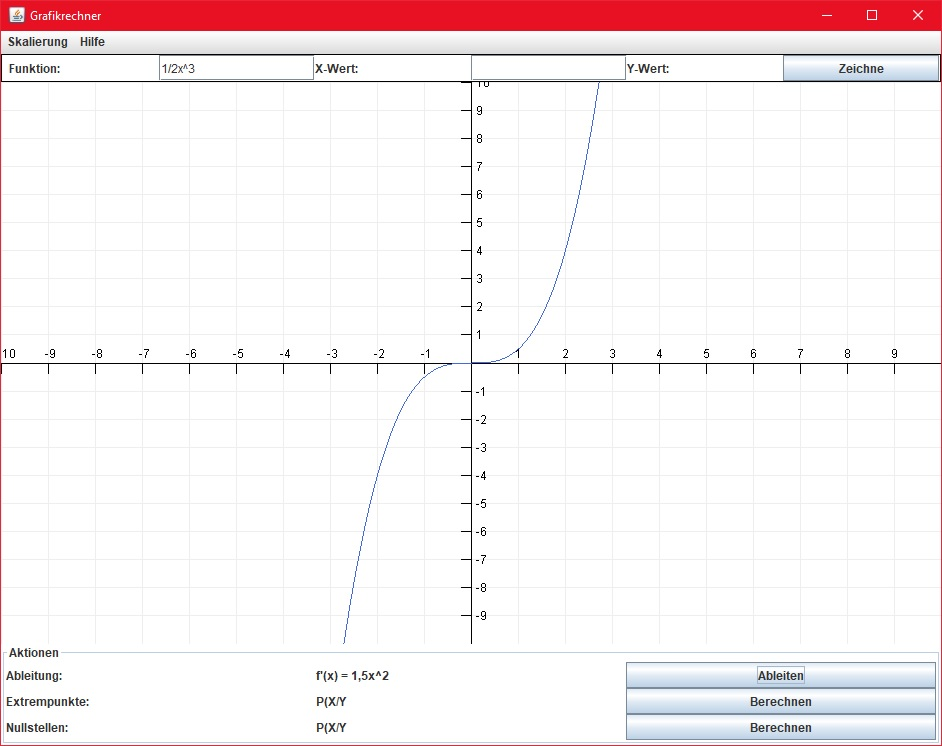
\includegraphics[width=1.0\textwidth]{Bilder/GR_1.jpg}
	\caption{Grafikrechner}
\end{figure}

\end{titlepage}


\tableofcontents
\newpage


%Ausgelagerte Elemente
%Vorwort

\ihead{\headmark}
\ohead{Lars Strölin, Michael Geigges, Ilja Kononenko}
\automark{section}
\cfoot{\pagemark}


\section{Vorwort}
Zu Beginn mussten wir uns zu dritt erst einmal zusammensetzen um zu besprechen was genau wir in unserem IT-Projekt erschaffen wollen. Die erste Frage war Android oder Java? Da wir alle mit Java schon mehr Erfahrung hatten und außerdem ein Programm für den PC erstellen wollten, war dies eine recht einfache Sache. Jetzt mussten wir nur noch wissen was für ein Programm wir erstellen und was dies können soll. 
\newline
Wir alle waren schon in der Lage mit Java Summen und andere mathematischen Formeln zu berechnen und hatten bereits einige Übungen, wie zum Beispiel da, wo wir unseren eigenen kleinen Taschenrechner mit den gewöhnlichen Aktionen Addition, Subtraktion, Multiplikation und Division programmiert haben. Dieses Mal sollte es aber etwas umfangreicheres werden und da wir in dem Fach "Mathe" gerade Funktionen behandelt haben, war unser erster Gedanke ein Programm welches bei Eingabe einer Funktion die entsprechende Grafik dazu anzeigt.
\newline
\newline
Diese Benutzerdokumentation beschreibt systematisch die Benutzung des Programms Grafikrechner. Diese sind in zwei Hauptthemen: Systeminformationen und Funktion gegliedert bzw. aufgeteilt.
Innerhalb der jeweiligen Themen werden mithilfe von Bildern erklärt, wie das Programm verwendet werden kann. Um die Bedienung der Programme so schnell wie möglich zu gewährleisten, sind die Beschreibungen deswegen so kurz wie möglich und kompakt gehalten worden. 




\newpage
%Softwareinformationen

\ihead{\headmark}
\ohead{Lars Strölin, Michael Geigges, Ilja Kononenko}
\automark{section}
\cfoot{\pagemark}


\section{Softwareinformationen}

\subsection{Installation}
Um das Programm auf einem PC zu benutzen benötigt man unsere selbst programmierte JAR-Datei und eine JAVA Version mit der Versionsnummer 1.8.0 oder höher. Nach einem Doppelklick auf die JAR-Datei öffnet sich das Programm und alles ist sofort voll funktionsfähig und benötigt keine weiteren Installationen. 



\subsection{Einführung}
Dieses PC-Programm ermöglicht einem oder mehreren Benutzern durch eine sehr übersichtliche und kompakte Oberfläche die Eingabe einer Ganzrationalen Funktion, die Anzeige der Funktion auf einem Koordinatensystem, sowie jeweils die Ableitung, die Berechnung der Extrempunkten und der Nullstellen. 
\newline
Zusätzlich können mit einem eingebauten Skalierungs-Menü die Skalierungswerte, also sprich X-Min, X-Max, Y-Min und Y-Max eingestellt werden, sodass man seine Funktion auf jeden Fall komplett sehen kann, oder bestimmte Punkte ganz gezielt durch den Zoom betrachten kann.
Eine weitere Funktion, die das Programm besitzt, ist das Anzeigen des Y-Wertes nach Eingabe einer Funktion mit einem X-Wert.



\newpage
%Funktion

\ihead{\headmark}
\ohead{Lars Strölin, Michael Geigges, Ilja Kononenko}
\automark{section}
\cfoot{\pagemark}


\section{Funktion}

\textbf{Funktionen und Aufbau im Überblick:}

\begin{enumerate}[label=\Roman*)]
	\item Eingabe
	\item Zeichnen
	\item Berechnen
	\item Hilfe
\end{enumerate}

%-----------------------------------------------------------------------------------------

\subsection{Eingabe}
Um eine Funktion eingeben zu können verwendet man das erste Eingabefeld links oben neben der Beschriftung "Funktion: ". Dort kann man dann eine X-beliebige Funktion eingeben, welche später auf dem KOS angezeigt werden kann.
\newline
Für die Berechnung eines Y-Wertes gibt es das zweite Eingabefeld rechts daneben mit der Beschriftung "X-Wert: ". Hier kann auch einen komplett beliebigen Wert mit einem "X" eingeben.

\begin{figure}[ht]
	\centering
	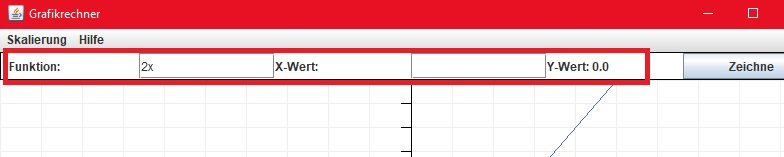
\includegraphics[width=1.0\textwidth]{Bilder/GR_2.jpg}
	\caption{Erstes und zweites Eingabefeld}
\end{figure}

%-----------------------------------------------------------------------------------------

\subsection{Zeichnen}
Um die Funktion dann auf dem Koordinatensystem anzeigen zu lassen benutzt man rechts oben im Eck den "Zeichne"-Button. Danach wird in anderer Farbe sofort auf dem Feld die Funktion gezeichnet und und korrekt angezeigt.

\begin{figure}[ht]
	\centering
	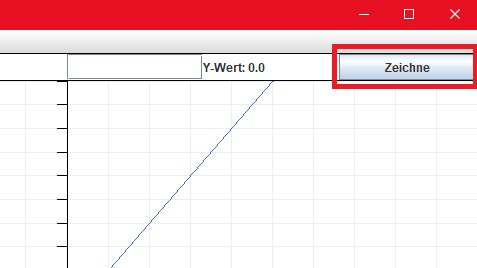
\includegraphics[width=0.6\textwidth]{Bilder/GR_3.jpg}
	\caption{Zeichne-Button}
\end{figure}


\subsubsection{Skalierung}
Die standardmäßige Größe des KOS (Koordinatensystem) beträgt in alle vier Richtungen 10 bzw. -10.
Aufgrund dessen, dass gewisse Funktionen ihre wichtigen Punkte in darüber liegenden Werten besitzen, oder der Benutzer einfach einen anderen Bereich gerne anschauen will, gibt es eine Einstellung für die Skalierung. 
\newline
In der Menüleiste gibt es links oben als erster Punkt das Menüitem Skalierung. Drückt man auf diesen Punkt öffnet sich ein Unterpunkt und unter dort kann man dann über ein Fenster, welches sich dann extra öffnet, die vier Werte der Skalierung manuell seinen Wünschen anpassen. Über den Punkt "Skalierung einstellen" werden die Werte auf der Anzeige übernommen. Der Punkt "Standard Skalierung" stellt die üblichen Werte 10 bzw. -10 wieder her.

\begin{figure}[ht]
	\begin{center}
		\subfloat[Menüitem Skalierung]{
		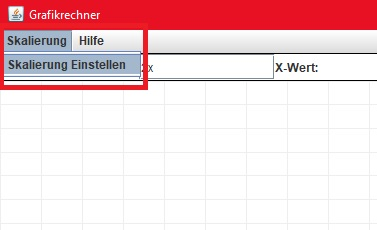
\includegraphics[width=0.4\textwidth]{Bilder/GR_4.jpg} }
	\hspace{1cm}
		\subfloat[Einstellungen für die Skalierung]{
		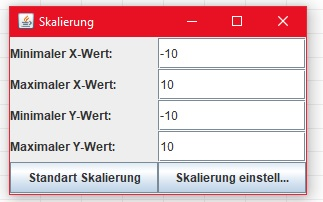
\includegraphics[width=0.4\textwidth]{Bilder/GR_5.jpg} }
	\end{center}
\end{figure}

%-----------------------------------------------------------------------------------------

\subsection{Berechnen}
Nach Eingabe einer Funktion im zweiten Eingabefeld gibt es rechts oben speziell für den Y-Wert ein Ausgabefeld. Um den Y-Wert zu erhalten muss man lediglich nach der Eingabe die "ENTER"-Taste drücken.

\subsubsection{Besondere Werte} 
In der Mathematik gibt es bestimmte Werte die von besonderer Bedeutung sind, wie z.B die Nullstellen, Hoch- und Tiefpunkte (Extrempunkte) oder die Ableitung. Auch dafür bietet das Programm unter dem KOS eine Lösung. Hier befinden sich jeweils drei Ausgabefelder mit einem "Berechne"-Button. Wird dieser nach einer korrekten Eingabe im ersten Eingabefeld gedrückt, werden die jeweiligen Werte berechnet und ausgegeben.

\begin{figure}[ht]
	\centering
	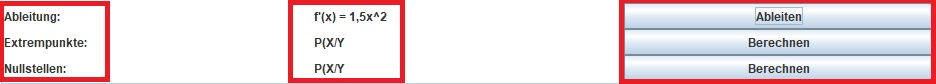
\includegraphics[width=1.0\textwidth]{Bilder/GR_6.jpg}
	\caption{Ausgabefelder für besondere Werte}
\end{figure}

\newpage

%-----------------------------------------------------------------------------------------

\subsection{Hilfe}
In der Menüleiste gibt es neben der Skalierung noch den zweiten Punkt "Hilfe". Dort kommt man zu den Unterpunkten "Anleitung" und "Über". 
\newline
Bei der Anleitung öffnet sich auch ein extra Fenster mit einer kleinen Anleitung um die Hauptfunktionen noch einmal zu erklären. 
\newline
Unter dem Punkt "Über" wird einem auch in ein einem extra Fenster die aktuelle Version des Programms und weitere Informationen angezeigt.

\begin{figure}[ht]
	\begin{center}
		\subfloat[Menüitem Hilfe]{
		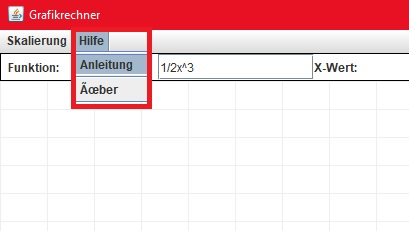
\includegraphics[width=0.4\textwidth]{Bilder/GR_7.jpg} }
	\hspace{1cm}
		\subfloat[Extrafenster für die Anleitung]{
		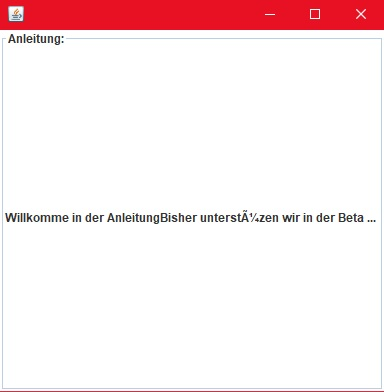
\includegraphics[width=0.4\textwidth]{Bilder/GR_8.jpg} }
	\end{center}
\end{figure}


%-----------------------------------------------------------------------------------------








\addcontentsline{toc}{section}{Stichwortverzeichnis}
\printindex

\end{document}